% 	%Template by Mark Jervelund - 2015 - mjerv15@student.sdu.dk

\documentclass[a4paper,10pt,titlepage]{report}



%Sensitive to import order.
\usepackage[dvipsnames]{xcolor}
\usepackage[utf8]{inputenc}
\usepackage[T1]{fontenc}
\usepackage[english]{babel}
\usepackage{amssymb}
\usepackage{amsmath}
\usepackage{amsthm}
\usepackage{graphicx}
\usepackage{fancyhdr}
\usepackage[normalem]{ulem}
\usepackage{lastpage}
\usepackage{multicol}
\usepackage{listings}
\usepackage{qtree}

\usepackage{cancel} 
\usepackage{algorithm}
\usepackage{algpseudocode}
\usepackage{subfig}
\usepackage{MnSymbol}
\usepackage[document]{ragged2e}
\usepackage[margin=1in]{geometry}
\usepackage{color}
\usepackage{datenumber}
\usepackage{venndiagram}
\usepackage{chngcntr}
\usepackage{enumitem}
\usepackage{mathtools}
\usepackage{tikz}
\usetikzlibrary{automata,positioning}
\DeclarePairedDelimiter{\ceil}{\lceil}{\rceil}

\title{DM553 - Notes}


\setdatetoday
\addtocounter{datenumber}{0} %date for dilierry standard is today
\setdatebynumber{\thedatenumber}
\date{}
\setcounter{secnumdepth}{0}
\pagestyle{fancy}
\fancyhf{}




%Commands

\newcommand\Ccancel[2][black]{\renewcommand\CancelColor{\color{#1}}\cancel{#2}}
\newcommand{\Z}{\mathbb{Z}}
\lhead{Complexity and Computability (DM553 - Notes))}
\rhead{Mark Jervelund (Mjerv15)}
\rfoot{Page  \thepage \, of \pageref{LastPage}}
\counterwithin*{equation}{section}








\begin{document}





\renewcommand{\thepage}{\roman{page}}% Roman numerals for page counter
\tableofcontents
\newpage
\setcounter{page}{1}
\renewcommand{\thepage}{\arabic{page}}
\section{Course description}
%%%%%%%%%%%%%%%%%%%%%%%%%%%%%%%%%%%%%%%%%%%%%
\newpage

\chapter{Exercises 2019}

\section{Week 1}

\subsection{page 84, question 1.7}

\subsubsection{a}

{w|w begins with a 1 and ends with a 0} \\
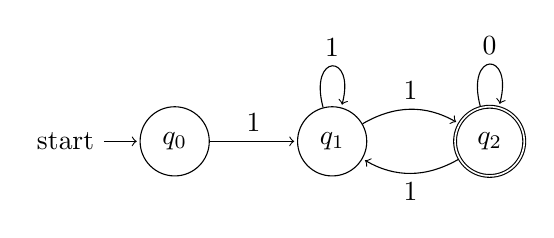
\begin{tikzpicture}[shorten >=1pt,node distance=2cm,on grid,auto] 
   \node[state,initial] (q_2)   {$q_0$}; 
   \node[state] (q_0)  [right=of q_2] {$q_1$}; 
   \node[state,accepting](q_1) [right=of q_0] {$q_2$};
    \path[->] 
    (q_0) edge [bend left]node {1} (q_1)
          edge [loop above] node {1} (q_0)
    (q_1) edge [bend left]node  {1} (q_0)
          edge [loop above] node {0} ()
    (q_2) edge node {1} (q_0);
\end{tikzpicture}


\subsubsection{b}
{w|w contains at least 3 1's}\\
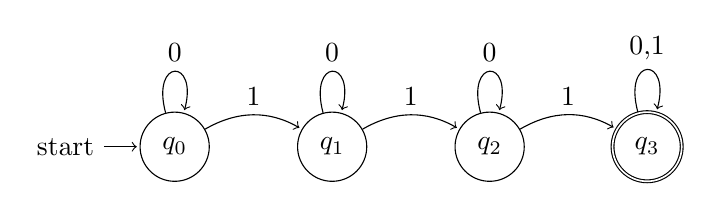
\begin{tikzpicture}[shorten >=1pt,node distance=2cm,on grid,auto] 
   \node[state,initial] (q_0)   {$q_0$}; 
   \node[state](q_1) [right=of q_0] {$q_1$};
   \node[state](q_2) [right=of q_1] {$q_2$};
   \node[state,accepting](q_3) [right=of q_2] {$q_3$};
    \path[->] 
    (q_0) edge [bend left]node {1} (q_1)
          edge [loop above] node {0} ()
    (q_1) edge [bend left]node  {1} (q_2)
          edge [loop above] node {0} ()
    (q_2) edge [bend left]node  {1} (q_3)
          edge [loop above] node {0} ()
    (q_3) edge [loop above] node {0,1} ();
\end{tikzpicture}


\subsubsection{c}
{w|w contains the substring 0101, (i.e. w = x0101y for some x and y)}
\\
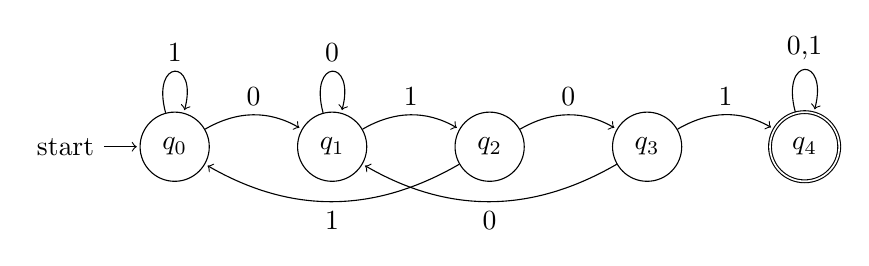
\begin{tikzpicture}[shorten >=1pt,node distance=2cm,on grid,auto] 
   \node[state,initial] (q_0)   {$q_0$}; 
   \node[state](q_1) [right=of q_0] {$q_1$};
   \node[state](q_2) [right=of q_1] {$q_2$};
   \node[state](q_3) [right=of q_2] {$q_3$};
      \node[state,accepting](q_4) [right=of q_3] {$q_4$};
    \path[->] 
    (q_0) edge [bend left]node {0} (q_1)
          edge [loop above] node {1} ()
          
    (q_1) edge [bend left]node  {1} (q_2)
          edge [loop above] node {0} ()
          
    (q_2) edge [bend left]node  {0} (q_3)
          edge [bend left] node {1} (q_0)
          
    (q_3) edge [bend left]node  {1} (q_4)
          edge [bend left] node {0} (q_1)
          
    (q_4) edge [loop above] node {0,1} ();
\end{tikzpicture}

\subsubsection{d}
{w|w bas at length of at least 3 and it's third symbol is 0}
\\
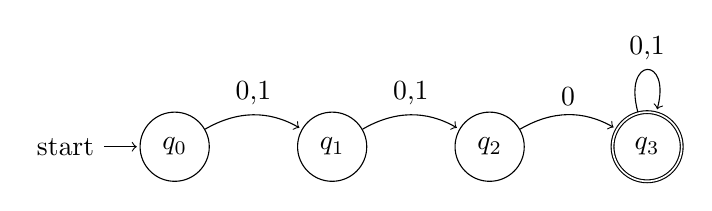
\begin{tikzpicture}[shorten >=1pt,node distance=2cm,on grid,auto] 
   \node[state,initial] (q_0)   {$q_0$}; 
   \node[state](q_1) [right=of q_0] {$q_1$};
   \node[state](q_2) [right=of q_1] {$q_2$};
   \node[state,accepting](q_3) [right=of q_2] {$q_3$};
    \path[->] 
    (q_0) edge [bend left]node {0,1} (q_1)
    (q_1) edge [bend left]node  {0,1} (q_2)
    (q_2) edge [bend left]node  {0} (q_3)
    (q_3) edge [loop above] node {0,1} ();
\end{tikzpicture}

\subsubsection{f}
{w|w doesn't contain the substring 001} \\
Accepts any string that doesn't contain the substring 001, and loops in rejecting state if this state is found, was unsure if the looping was needed but included it if it was the case.\\
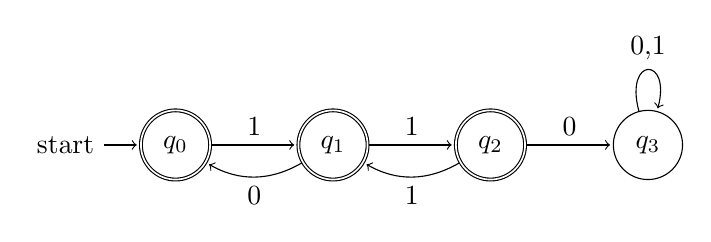
\begin{tikzpicture}[shorten >=1pt,node distance=2cm,on grid,auto] 
   \node[state,initial,accepting] (q_0)   {$q_0$}; 
   \node[state,accepting](q_1) [right=of q_0] {$q_1$};
   \node[state,accepting](q_2) [right=of q_1] {$q_2$};
   \node[state](q_3) [right=of q_2] {$q_3$};
    \path[->] 
    (q_0) edge node {1} (q_1)
    (q_1) edge node  {1} (q_2)
          edge [bend left] node {0} (q_0)
    (q_2) edge node  {0} (q_3)
    	edge [bend left] node {1} (q_1)
    (q_3) edge [loop above] node {0,1} ();
\end{tikzpicture}
\\

\subsubsection{h}
{w|w is any string except 11 and 111}\\
accepts any string that isn't 11, 111 including the empty string $\epsilon $ \\
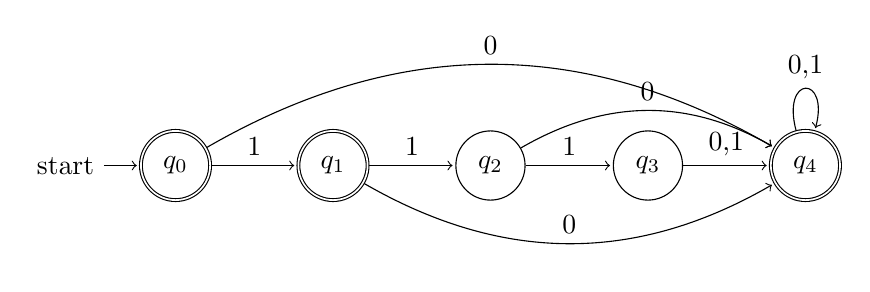
\begin{tikzpicture}[shorten >=1pt,node distance=2cm,on grid,auto] 
   \node[state,initial,accepting] (q_0)   {$q_0$}; 
   \node[state,accepting](q_1) [right=of q_0] {$q_1$};
   \node[state](q_2) [right=of q_1] {$q_2$};
   \node[state](q_3) [right=of q_2] {$q_3$};
   \node[state,accepting](q_4) [right=of q_3] {$q_4$};
    \path[->] 
    (q_0) edge node {1} (q_1)
   		  edge [bend left] node {0} (q_4)
    (q_1) edge node  {1} (q_2)
    	  edge [bend right] node {0} (q_4)
    (q_2) edge node  {1} (q_3)
    	  edge [bend left] node {0} (q_4)
    (q_3) edge node {0,1} (q_4)
    (q_4) edge [loop above] node {0,1} ();
\end{tikzpicture}

\subsubsection{i}
{w|w every odd position of w is a 1} \\
accepts all states where \#1\#1\#1\#1\#1 is followed also accepts the empty string $ \epsilon $ \\


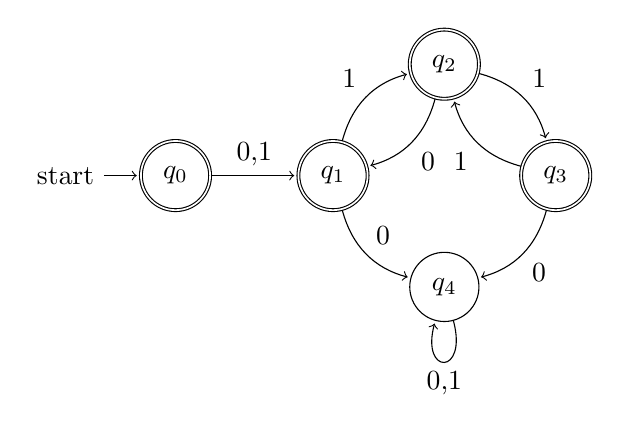
\begin{tikzpicture}[shorten >=1pt,node distance=2cm,on grid,auto] 
   \node[state,initial,accepting] (q_0)   {$q_0$}; 
   \node[state,accepting](q_1) [right=of q_0] {$q_1$};
   \node[state,accepting](q_2) [above right=of q_1] {$q_2$};
   \node[state](q_4) [below right=of q_1] {$q_4$};
   \node[state,accepting](q_3) [above right=of q_4] {$q_3$};
    \path[->] 
    (q_0) edge node {0,1} (q_1)
    (q_1) edge [bend left]node  {1} (q_2)
          edge [bend right] node {0} (q_4)
    (q_2) edge [bend left] node  {1} (q_3)
    	  edge [bend left] node {0} (q_1)
    (q_3) edge [bend left] node {0} (q_4)
   		  edge [bend left] node {1} (q_2)
   	(q_4) edge [loop below] node {0,1} ();
\end{tikzpicture}


\subsubsection{k}
{w|w is only the empty string and 0} \\
accepts "0" and the empty string $ \epsilon $ \\


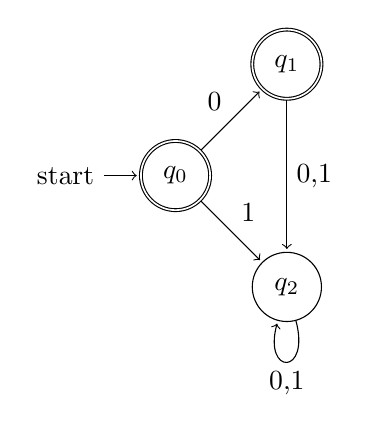
\begin{tikzpicture}[shorten >=1pt,node distance=2cm,on grid,auto] 
   \node[state,initial,accepting] (q_0)   {$q_0$}; 
   \node[state,accepting](q_1) [above right =of q_0] {$q_1$};
   \node[state](q_2) [below right =of q_0] {$q_2$};

    \path[->] 
    (q_0) edge node {0} (q_1)
    	  edge node  {1} (q_2)
    (q_1) edge node {0,1} (q_2)
   	(q_2) edge [loop below] node {0,1} ();
\end{tikzpicture}

\newpage
\subsection{page 84, question 1.7}

\subsubsection{d}
The language {0} with two states,\\

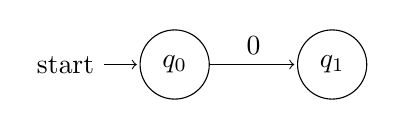
\begin{tikzpicture}[shorten >=1pt,node distance=2cm,on grid,auto] 
   \node[state,initial] (q_0)   {$q_0$}; 
   \node[state](q_1) [right =of q_0] {$q_1$};

    \path[->] 
    (q_0) edge node {0} (q_1);
\end{tikzpicture}
\subsubsection{e}
the language 0*1*0* with 3 states \\
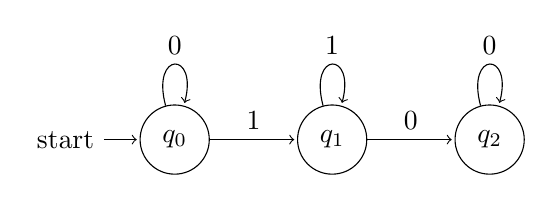
\begin{tikzpicture}[shorten >=1pt,node distance=2cm,on grid,auto] 
   \node[state,initial] (q_0)   {$q_0$}; 
   \node[state](q_1) [right =of q_0] {$q_1$};
   \node[state](q_2) [right =of q_1] {$q_2$};

    \path[->] 
    (q_0) edge node {1} (q_1)
    	edge [loop above]node  {0} (q_2)
    (q_1) edge node {0} (q_2)
    edge [loop above]node  {1} (q_2)
   	(q_2) edge [loop above]node  {0} (q_2);
\end{tikzpicture}
\subsubsection{g}
the language {$\epsilon$} with 1 state \\

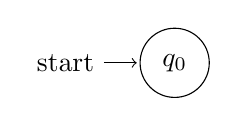
\begin{tikzpicture}[shorten >=1pt,node distance=2cm,on grid,auto] 
   \node[state,initial] (q_0)   {$q_0$}; 
\end{tikzpicture}


\subsubsection{h}
The language 0* with 1 state \\

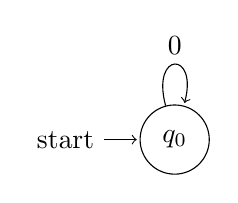
\begin{tikzpicture}[shorten >=1pt,node distance=2cm,on grid,auto] 
   \node[state,initial] (q_0)   {$q_0$}; ;

    \path[->] 
    (q_0) [loop above]edge node {0} ();
\end{tikzpicture}


\subsection{Solve the following problem,}

A man is travelling with a wolf (w) and a goat (g). He also brings along a nice big
cabbage (c). He encounters a small river which he must cross to continue his travel.
Fortunately, there is a small boat at the shore which he can use. However, the boat
is so small that the man cannot bring more than himself and exactly one more item
along (from {w, g, c}). The man knows that if left alone with the goat, the wolf will
surely eat it and the goat if left alone with the cabbage will also surely eat that. The
man’s task is hence to device a transportation scheme in which, at any time, at most
one item from {w, g, c} is in the boat and the result is that they all crossed the river
and can continue unharmed.

\subsubsection{a} Describe a solution to the problem which satisfies the rules of the “game”. You may use your answer to (b) to find a solution. \\

\begin{itemize}
\item First you carry the goat to the other side, and go back empty.
\item The you ferry the wolf to the other side, and swap with the goat and bring the goat back.
\item you then swap the goat with the cabbage and bring it to the other side.
\item lastly you head back empty and bring the goat.
\item you now have all the items on the other side of the river.
\end{itemize}


\subsubsection{b}
The string all of the valid moves are 
\begin{equation}
\begin{split}
(g(m(x(g(y(m(g)*)*)*)*)*)*)* \\
x,y = (w|c) \\
x \neq y
\end{split}
\end{equation}


\vspace{5mm}
This is due to the fact that it's legal moves in the game, like the man can bring the goat to the other side and bring it back too, it's bad move, but it's still a valid move. \\

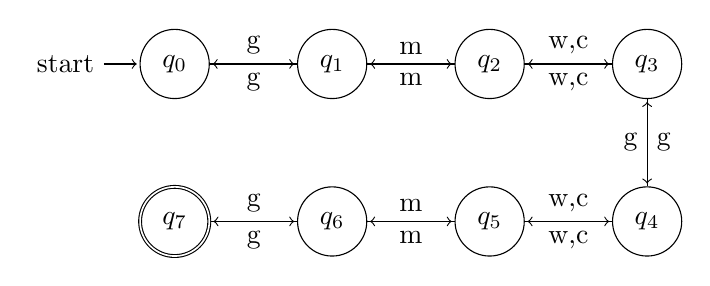
\begin{tikzpicture}[shorten >=1pt,node distance=2cm,on grid,auto] 
   \node[state,initial] (q_0)   {$q_0$}; 
   \node[state](q_1) [right =of q_0] {$q_1$};
   \node[state](q_2) [right =of q_1] {$q_2$};
   \node[state](q_3) [right =of q_2] {$q_3$};
   \node[state](q_4) [below =of q_3] {$q_4$};
   \node[state](q_5) [left =of q_4] {$q_5$};
   \node[state](q_6) [left =of q_5] {$q_6$};
   \node[state,accepting](q_7) [left =of q_6] {$q_7$};

    \path[->] 
    (q_0) edge node {g} (q_1)
    (q_1) edge node {g} (q_0)
   	      edge node {m} (q_2)
    (q_2) edge node {m} (q_1)
   	      edge node {w,c} (q_3)
   	(q_3) edge node {w,c} (q_2)
   	      edge node {g} (q_4)
   	(q_4) edge node {g} (q_3)
   	      edge node {w,c} (q_5)
   	(q_5) edge node {w,c} (q_4)
   	      edge node {m} (q_6)
   	(q_6) edge node {m} (q_5)
   	      edge node {g} (q_7)   	      
   	(q_7) edge node {g} (q_6);
\end{tikzpicture}




\section{Week 2}

\subsection{page 86, question 1.16}
* is any number \\
! is one or more \\

\subsubsection{a}
it accepts (bb)*a!(a|b)* \\

the language 0*1*0* with 3 states \\
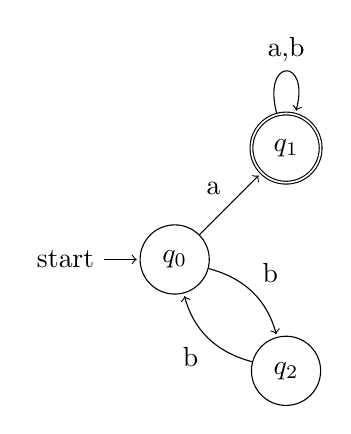
\begin{tikzpicture}[shorten >=1pt,node distance=2cm,on grid,auto] 
   \node[state,initial] (q_0)   {$q_0$}; 
   \node[state,accepting](q_1) [above right =of q_0] {$q_1$};
   \node[state](q_2) [below right =of q_0] {$q_2$};

    \path[->] 
    (q_0) edge node {a} (q_1)
   		  edge [bend left]node {b} (q_2)
    (q_1) edge [loop above]node {a,b} (q_1)
   	(q_2) edge [bend left]node  {b} (q_0);
\end{tikzpicture}

\subsubsection{b}


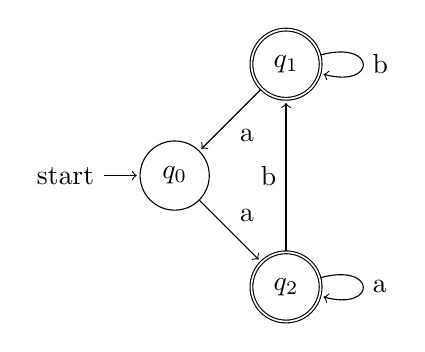
\begin{tikzpicture}[shorten >=1pt,node distance=2cm,on grid,auto] 
   \node[state,initial] (q_0)   {$q_0$}; 
   \node[state,accepting](q_1) [above right =of q_0] {$q_1$};
   \node[state,accepting](q_2) [below right =of q_0] {$q_2$};

    \path[->] 
    (q_0) edge node {a} (q_2)
   		  
    (q_1) edge node {a} (q_0)
    	  edge [loop right]node {b} ()
   	(q_2) edge [loop right]node  {a} ()
   	      edge []node  {b} (q_1);
\end{tikzpicture}

\subsection{page 86, question 1.17}

\subsubsection{a}
The first task is to make a NFA recognizing (01u001u010)* \\
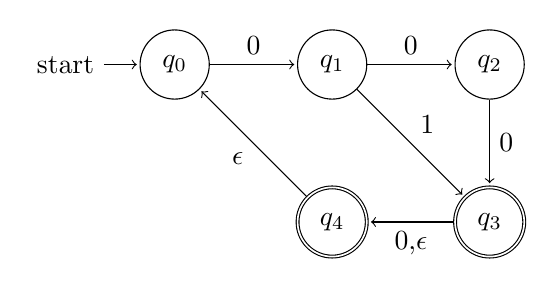
\begin{tikzpicture}[shorten >=1pt,node distance=2cm,on grid,auto] 
   \node[state,initial] (q_0)   {$q_0$}; 
   \node[state](q_1) [right =of q_0] {$q_1$};
   \node[state](q_2) [right =of q_1] {$q_2$};
   \node[state,accepting](q_3) [below =of q_2] {$q_3$};
   \node[state,accepting](q_4) [below =of q_1] {$q_4$};



    \path[->] 
    (q_0) edge node {0} (q_1)
    (q_1) edge node {0} (q_2)
    	  edge node {1} (q_3)
   	(q_2) edge node {0} (q_3)
   	(q_3) edge node {0,$\epsilon$} (q_4)
   	(q_4) edge node {$\epsilon$} (q_0);
\end{tikzpicture}
\\

\subsubsection{b}
After converting this to a DFA\\

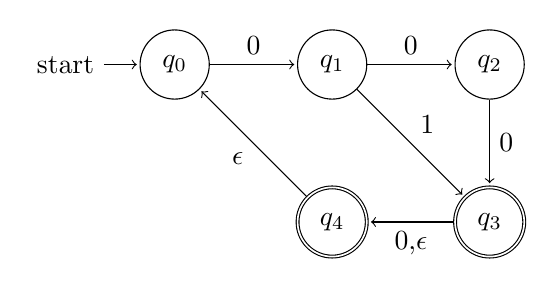
\begin{tikzpicture}[shorten >=1pt,node distance=2cm,on grid,auto] 
   \node[state,initial] (q_0)   {$q_0$}; 
   \node[state](q_1) [right =of q_0] {$q_1$};
   \node[state](q_2) [right =of q_1] {$q_2$};
   \node[state,accepting](q_3) [below =of q_2] {$q_3$};
   \node[state,accepting](q_4) [below =of q_1] {$q_4$};



    \path[->] 
    (q_0) edge node {0} (q_1)
    (q_1) edge node {0} (q_2)
    	  edge node {1} (q_3)
   	(q_2) edge node {0} (q_3)
   	(q_3) edge node {0,$\epsilon$} (q_4)
   	(q_4) edge node {$\epsilon$} (q_0);
\end{tikzpicture}

\subsection{page 86, question 1.18}
Predefined terms
\begin{equation}
x = (0,1)^*
\end{equation}
\begin{equation}
y = (0|1)
\end{equation}

\subsubsection{a}
$1x0$
\subsubsection{b}
$x1x1x1x$
\subsubsection{c}
$x0101x$
\subsubsection{d}
$yy0x$
\subsubsection{e}
$(0(yy)*)|1y(yy)^*)$
\subsubsection{f}
$ 0^*(1+10)^* $
\subsubsection{g}
$ yyyyy $


\subsection{page 86, question 1.19 a}

Convert the following regex to a NFA via lemma 1.55\\
\begin{equation}
(0 \cup 1)^*000(0\cup 1)^* 
\end{equation}
\begin{center}


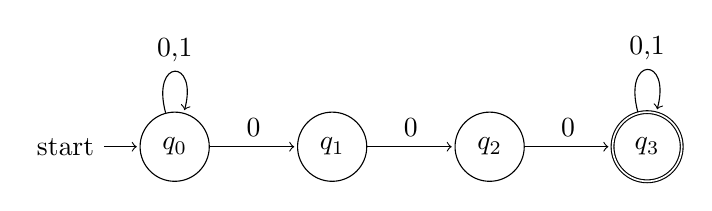
\begin{tikzpicture}[shorten >=1pt,node distance=2cm,on grid,auto] 
   \node[state,initial] (q_0)   {$q_0$}; 
   \node[state](q_1) [right =of q_0] {$q_1$};
   \node[state](q_2) [right =of q_1] {$q_2$};
   \node[state,accepting](q_3) [right =of q_2] {$q_3$};



    \path[->] 
    (q_0) edge [loop above] node {0,1} (q_0)
    	  edge node {0} (q_1)
    (q_1) edge node {0} (q_2)
   	(q_2) edge node {0} (q_3)
   	(q_3) edge [loop above] node {0,1} ();
\end{tikzpicture}
\end{center}

\subsection{page 86, question 1.20}
For each of the following expressions give two strings that are and two that are not in the languages. assume that the alphabet is \{a,b\}
\begin{multicols}{2}
\subsubsection{a}
\begin{equation}
a^*b^*
\end{equation}
member\\
aa, ab, aabb, aab, abbbb\\
not member\\
ba, abab, \\
\subsubsection{b}
\begin{equation}
a(ba)^*b
\end{equation}
member\\
abab, ababababab,\\
not member\\
aaba baba\\
\subsubsection{c}
\begin{equation}
a^* \cup B^*
\end{equation}
member\\
ab, aabb \\
not member \\
ba, aabba\\
\subsubsection{d}
\begin{equation}
(aaa)^*
\end{equation}
member\\
aaa, aaaaaa \\
not member\\
a, aaaa\\
\subsubsection{e}
\begin{equation}
\sum^*a\sum^*b\sum^*a\sum^*
\end{equation}
member\\
todo\\
not member\\
todo\\
\subsubsection{f}
\begin{equation}
aba \cup bab
\end{equation}
member \\
todo\\
not member\\
todo\\
\subsubsection{g}
\begin{equation}
(\epsilon \cup a)b
\end{equation}
member\\
ab, b\\
not member\\
abb, aab\\
\subsubsection{h}
\begin{equation}
(a\cup ba \cup bb)\sum^*
\end{equation}
member\\
todo\\
not member\\
todo \\
\end{multicols}
\subsection{page 86, question 1.21 b}

The solution is 
\begin{equation}
((a|b)(a,bb)*b(a)?)*
\end{equation}
(a or b, followed by any number of (a,bb)* followed by a single b (as it matches uneven numbers of b and followed by 0 or 1 a*

\subsection{page 86, question 1.29}

\subsubsection{a}

For the task a we have the sting 
\begin{equation}
0^n1^n2^n
\end{equation}
the first contradiction is that when we have a string eg. 000111222 and we split it so we have the floowing, x = 000, y = 111, z = 222 and we pump y so we have the string xyyz this violates the first condition of the pumping lemma, as we'll have more 1s then 0s and 2s.

the string y only contains 1s which also causes a contradiction.

and the 3rd case if we have the string x = 00, y = 011 and z = 1222 where we'll get out of order letters so we'll again reach a contradiction.


\subsubsection{b}

For assignment b i find it a bit odd, i may misunderstand the exercise but w/e

We want to pump the language
\begin{equation}
a_2 = \{www|w \in \{a,b\}^*\}
\end{equation}
But from my understanding is the * a kleen star? eg then one w and www are equivalent as \{a,b\} is all possibly strings in the library w. ? or is it understand such that w is equal to either a or b but any number of them eq $\{a|b\}^*$,\\
How i choose to intercept it for now is that w is equal to either the string a* or b* and if this is the case then some of the same argumentation as for task a is valid.
\\
www can give us the string 111000111 and we can split it as follows. 111|1000|11111, This means that zyyx gives of a out of order 1 and we therefor get a contradiction wrt. to the pumping lemma.


\subsection{page 88, question 1.30}
The error There's a few things here, the first case from 1:73 fail right away as the string 0001111 is in the lang, the case of out of order fails as if we can get the string 00100111 ten we'll reach a contradiction but the case of 



\subsection{page 89, question 1.36}

For the language w there exist a DFA that accepts if, for the revere language $w^r$ the DFA which a reversed edges and the start state is now our accept state. 


\section{week 3}

\subsection{page 88, question 1.29(a),(b) and 1.30}

Already done, see above.

\subsection{page 89. question 1.35}
\textbf{ILONA}
As B is in bijection of A there for it's a regular.


\subsection{page 91. question 1.51}
\begin{multicols}{2}


\subsubsection{a}
This can be proved via the pumping lemma. where you can get out of order 1 and/or 0s and that causes a contradiction.

\subsubsection{b}
Same as a wrt. our of order.

\subsubsection{c}

This is this is either the unbounded string 0 or 1.

\subsubsection{d}
this is again wrt. out of order 0.1 eg. if we can get the string 01010 by umping as this is not in the lang.
\end{multicols}
\subsection{page 154. question 2.2}
Give parse trees and derivations for each string using the following Context free gramma (CFG)  \\
\begin{center}
$ E \rightarrow E+T | T$ \\
$ T \rightarrow E \times F | F $ \\
$ F \rightarrow (E) | a$
\end{center}


\begin{figure}[h]%
    \centering
    \subfloat[a]{{\Tree[.E [.T [.F [a ]]]] }}%
    \qquad
    \subfloat[a+a]{{\Tree
	[.E 
		[.T [.F [a ]]]
		+Manuelly
		[.E [.T [.F [a ]]]]
	] }}%
	\qquad
    \subfloat[a+a+a]{{
    \Tree
	[.E 
		[.T [.F [a ]]]
		+
		[.E [.T [.F [a ]]]
			+
			[.E [.T [.F [a ]]]		
		]
	]]
	}}%
	    \subfloat[((a))]{{
	\Tree
	[.E 
		[.T [.F [( [.E [.T [.F [( [[.T [.F [a ]]]] ) ]]]] ) ]]]
	]
	}}%
    \caption{2 Figures side by side}%
    \label{fig:example}%
\end{figure}

\subsection{page 154. question 2.4}
\begin{multicols}{2}
\subsubsection{a}
$ S \rightarrow TTT $\\
$ T \rightarrow E1E $\\
$ E \rightarrow FTF $\\
$ F \rightarrow 0 | \epsilon $\\
\subsubsection{b}
$ S \rightarrow 0F0 | 1F1 $\\
$ F \rightarrow F0F | F1F | \epsilon $\\
\subsubsection{c}
$ S \rightarrow EFE $\\
$ E \rightarrow FEF | EFF | FFE | \epsilon $\\
$ F \rightarrow 0 | 1$
\subsubsection{d}
$ S \rightarrow E0E $\\
$ E \rightarrow FEF | \epsilon $\\
$ F \rightarrow 0 | 1$
\subsubsection{e}
$ S \rightarrow E $\\
$ E \rightarrow FEF | GEG | \epsilon $\\
$ F \rightarrow 0 $
$ G \rightarrow 1 $
\subsubsection{f}
$ S \rightarrow \epsilon $ \\


\end{multicols}
\newpage
\subsection{2.6}
Give the CFG that generates the following languages
\begin{multicols}{2}

\subsubsection{b}
The complment of the langauges $ \{a^nb^n | n \geq 0 \} $

$ S \rightarrow FG $\\
$ G \rightarrow GbG $\\
$ F \rightarrow FaF $

\subsection{d}
For the third one it's a unbounded string with up to k alternations of $0^*1^*0^*1^*0^*$

This can simply be defined using the following grammar.

$ S \rightarrow FG $\\
$ E \rightarrow GE | FE | \epsilon $\\
$ G \rightarrow 1G | \epsilon $\\
$ F \rightarrow 0F | \epsilon $

\end{multicols}


\subsection{2.14}
We start in the initial state \\
$ A \rightarrow BAB | B | \epsilon $\\
$ B \rightarrow 00 | \epsilon $ \\
\vspace{5mm}
From here we put a new start state S\\
\vspace{5mm}
$ S \rightarrow A$\\
$ A \rightarrow BAB | B | \epsilon $\\
$ B \rightarrow 00 | \epsilon $\\
\vspace{5mm}
From here we can eliminate the first $\epsilon$ \\
\vspace{5mm}
$ S \rightarrow A$\\
$ A \rightarrow BAB | B | \epsilon \textcolor{OliveGreen}{|BA|AB}$\\
$ B \rightarrow 00 $ $\textcolor{OliveGreen}{\cancel{ | \ \epsilon \ }}$\\

From here we can eliminate the $\epsilon$  in our 2nd rule, \\
\vspace{5mm}
$ S \rightarrow\Ccancel[red]{ | \ A \ |} \textcolor{red}{ BAB|\Ccancel[Cyan]{ B |}BA|AB|\epsilon} \textcolor{Cyan}{|CC}$\\
$ A \rightarrow BAB | \Ccancel[Cyan]{ B |} {\Ccancel[red]{  \ \epsilon \ |}} \textcolor{OliveGreen}{BA|AB} \textcolor{Cyan}{|CC}$\\
$ B \rightarrow \Ccancel[Cyan]{ 00 |}  \Ccancel[OliveGreen]{ \epsilon | } CC$\\
$ \textcolor{Cyan}{C -> 0} $
\subsection{page 156, question 2.16}
Show that the class of context free languages are closed under the regular operations Concatenation, union and Star\\ 
Using the following grammar \\
\begin{itemize}
\item $ S_1 \rightarrow aS_1b$
\item $ S_1 \rightarrow \epsilon$

\item $ S_2 \rightarrow cS_2d$
\item $ S_2 \rightarrow \epsilon$
\end{itemize}
\subsubsection{Concatenation}
This is simply shown via 

Making s start symbol S, and have the two languages follow each other $S_1$ $S_2$ \\
$S \rightarrow S_1S_2$
\subsubsection{Union}
This is simply shown via 

Making s start symbol S, \\
$S \rightarrow S_1 | S_2$
\subsubsection{Star}
This is simply shown via 

Making s start symbol S, \\
$S \rightarrow S_1S$


\subsection{page 158, question 2.32}
 Let $A/B=\{w|wx \in A$ for some $x \in B \}$, Show that if A is context free and B is regular, then A/B is context free.
 
 "Proof. We can augment the memory of the PDA recognizing the CFL with the DFA recognizing the regular langauge and run both machines in parallel. We accept iff both machines accept.\ref{http://web.mit.edu/bmhuang/www/notes/18404-notes.pdf page 14, 4.3}\\
 note the intersection of two CFL's and not necessarily a CFL.!
 
 
 \subsection{page 158, question 2.38}
 As each step has a most 2 sub rules we can calculate that at step 1 we increasing the string length by 2n-1 and as all rules do this our end case is 2n-1
 
 \subsection{page 158, question 2.42}
 • 2.42 Hint for (d): first intersect the language with a suitably chosen regular language
and then prove that the language you obtain is not context-free.

 \begin{multicols}{2}
\subsubsection{a}
A break wrt. out of order letters, and not n counts of some letter
\subsubsection{b}
For the lang b is has to be in the size of wrt. $n+n^2+n^3$ eg 3,14, 39, 84, 155 and you can pump it to a length not in this range,

\subsubsection{c}
i dont know
\subsubsection{d}
i dont know

\end{multicols}
\newpage
\section{week 4}

\subsection{2.58}

let $\sum = \{0,1\}$ and let B be the collection of strings that contain at least one 1 in their second half, in other words,$ B = \{uv | u \in \sum ^*, v \in \sum^* 1 \sum^*$ and $ |u| \geq |v|\}$
\\
\subsubsection{a}
 Give a PDA that recognizes B
 
$ S \rightarrow XTX | X1$ \\
$ T \rightarrow XT | X $ \\
$ X \rightarrow 1|0$ \\
 
 
 \subsubsection{b}
Give a CFG that generates B
Read the input from end to front, pushing every 0 you meet onto the stack. if a 1 is found you continue parsing but instead pop a letter from the stack until it's empty, if you reach the beginning of the input before the stack is empty you reject.

\subsection{2002 program 2}
Let $\sum$ be a finite alphabet and let $L \subset \sum^+ $ be a regular language, Define a new language L'as the language of all words w $\in \sum^*$ such that w is obtained from a word in L by deleting the first letter, is the language L' regular as well? prove your answer\\





\newpage
\chapter{Questions 2018}
\newpage
\section{1. Finite automata and regular languages}

\subsection{Introduction}
I'm going to talk about Finite automata and regular languages.

\subsubsection{Finite automata}
	Finite automata is the simplest computational model that works via states and transitions, and therefor uses extremely limited memory. Using this model we can recognize and formulate regular languages, This can be a simple tasks a finding a substring, or used as a tool for designing more complex systems. \\
	
A Finite atomata is defined as a tuple containing the set of states Q, The known alphabet $\sigma$, The transition function $\delta: Q \times \sigma \longrightarrow Q$the start state $q_1$ and the set of accept states F. \\
	
\subsubsection{Regular languages}
	A regular languages is a sequence of letters in some alphabet defined by $\sum$ the empty alphabet is defined by the empty set $ \emptyset $, and contains letters and the empty string $ \epsilon $. they are also closed under the union $ \cup $, concatination $ \cap $, and kleene star $^*$, and the proceeding order is $^*, \cap, \cup$, A language is Regular is a Finite automata recognizes it.
	
\subsection{Pumping lemma for regular languages}

The pumping lemma is a way for us to proof if a language is regular. The theorem for the pumping lemma states that the 3 conditions for the lemma is\\
\begin{itemize}
\item for each $i \geq 0, xy^iz \in A $
\item $ |y| > 0 $
\item $ |xy| \leq p$ where p is the pumpking length. 
\end{itemize} 


$0^n1^n | n \geq 0$

The way you do this is to assume it's regular and make a counter argument. with the pumping lemma we have 3 conditions that our counter argument most meet. the first case we can pump the language to have more 1's than 0s or(2) the other way around.. the third(3) is that we can get out of order letters if we pump a string containing both 0s and 1s, 
	
\subsection{Deterministic And Non-deterministic}

The difference between deterministic and non-deterministic is the way they operate. they recognize the same class of languages as a NFA can be  convert into a DFA and the same goes the other way around, it is not a efficiency operation as the algorithm is exponential. there is however some benefits to both. where the non-deterministic preforms branching and could potentially benefit the execution wrt. size, runtime. or recourse consumption. \\

The correct term here would that that a DFA Can simulate a NFA \\


\newpage
\section{2. Pushdown automata and context-free languages}


\subsection{Introduction}
I'm going to talk about Pushdown automata and context free languages. These topics are used in modern compilers to parse a programming language and is a useful tool in language processing wrt. human language as well as when interpreting one language to an other.
\subsection{Pushdown automata}
A pushdown automata is a type of automaton that employs a stack to help with the computation, this allows the PDA to recognize and run Context free grammars and all the languages below it.
\subsection{Context free grammar}
A CFG consist of a collection of substitution rules, a CFG operate on a set of variables, terminals and a designated start symbol.
 an exsample of such a rule is:
 $A \rightarrow 0A1$\\
 $A \rightarrow B$\\
 $B \rightarrow \# $ \\
 
This above gramma should generate the string $0^n\#1^n$ where n is any natural number including 0.\\

The formal definistion of a CFG is a 4 tuple consisting of the set of variables V, the set of terminals $\sum$, the set of rules R and the start symbol S that is in V\\

A more advanced example could be the over the set of variables and terminals \{num,A,-\}\\
Lets say we have the following rules \\
$A \rightarrow A-A $\\
$A \rightarrow num$\\

for the above grammar if we apply it to the grammar\\
1-2-3 we can get the output 2 or -4 depending on how the grammar is parsed. (1-2)-3 vs 1-(2-3)\\
We can handle this ambiguity in two manners either we introduce the terminals ( and ) to the language or we can rewrite or rules as to not have this bias.\\
\subsection{Chomsky normal Form}
Chomsky normal form is a simplified form that we can convert our grammars into which enables to decide things like if a string is generated by a grammar in polynomial time. \\

The steps to convert a gramma to CNF is to:\\
\begin{enumerate}
\item eliminate all $\epsilon$ productions.
\item Eliminate all productions where RHS is one variable
\item Eliminate all productions longer than 2 variables
\item move all terminals to productions where RHS is one terminal.
\end{enumerate}


\subsection{Pumping lemma of CFL}




\newpage
\section{3. Turing machines}

Introduction
    What is a turning machine
        
Multitape

Nondetermanistic turning machine
    Faster but less powerfull?
    



\newpage
\section{4. Decidability}
Introduction
 If a language  defined by a DFA is decidable.


Examples of Decidability and undecidability




\newpage
\section{5. Reducibility}
What is it and how to use it.





\newpage
\section{6. NP-completeness proofs – examples.}
what is np\_completeness

Why we use it to reduce,

Proff of np complete.
qlique, subset sum, Hamiltonian circuit, 




\newpage
\section{7. Proof that SATISFIABILITY is NP-complete (do not assume that
there is a known NP-Complete problem — use the proof in Sipser’s
book).}

Cook-levin theorem - insipset, præsentation use slides on homepage.
\newpage
\section{8. Information-theoretic lower bounds (lower bounds proven by counting
leaves in decision trees), especially the average case bounds for sorting
by comparisons.}
As is average case.




\newpage
\section{9. Adversary arguments – technique, examples.}





\newpage
\section{10. Median problem – algorithm and lower bound.}





\newpage
\section{11. Approximation algorithms}

vertex cover

 
\end{document}




%
%
%
% Old STOP!, This is the "trash"
% 
%


%%%%%%%%%%%%%%%%%%%%%%%%%%%%%%%%%%%5
\newpage
\chapter{Questions 2017}
\section{Questions from last year}
1. Finite automata and regular languages \\
2. Pushdown automata and context-free languages\\
3. Turing machines\\
4. Decidability\\
5. Reducibility\\
6. NP-completeness proofs – examples.\\
7. Proof that SATISFIABILITY is NP-complete.\\
8. Information-theoretic lower bounds (lower bounds proven by counting leaves in decision trees), especially the average case bounds for  sorting by comparisons.\\
9. Adversary arguments – technique, examples.\\
10. Approximation algorithms.\\
\newpage
\subsection{1. Finite automata and regular languages}
\subsubsection{Introduction}
\subsubsection{Types of Automata}
	DFA - 
    NDFA - 

\newpage
\subsection{2. Pushdown automata and context-free languages}
	CFG(context free grammar)
    	regular language
        	defined by DFA
           ambiguity
           		inherited ambiguity
           Chomsky normal form
           		You're allowed to have a rule that turns A into two sub rules.
           			A -> BC
                You can have a rule about a terminal set for our alphabet.
                	$A -> a \in \sum \epsilon $
                You're only allowed to produce Epsilon from the start symbol.
                	$S -> \epsilon $
            theorem
            	Any CFL is generated by a CFG in Chomsky normal form,
                
    pushdown automata PDA(s) 
    		NFA with a stack.
    	
    	
           
\subsection{3. Turing machines}
\subsection{4. Decidability}
\subsection{5. Reducibility}
\subsection{6. NP-completeness proofs – examples.}
\subsection{7. Proof that SATISFIABILITY is NP-complete.}
\subsection{8. Information-theoretic lower bounds (lower bounds proven by counting leaves in decision trees), especially the average case bounds for sorting by comparisons.}
\subsection{9. Adversary arguments – technique, examples.}
\subsection{10. Approximation algorithms}

%
\newpage
\chapter{Lectures}
\subsection{Format}
Titles should be listed as (date - topic(s)) for easier lookup

\subsection{28-feb-2018 - TBD}
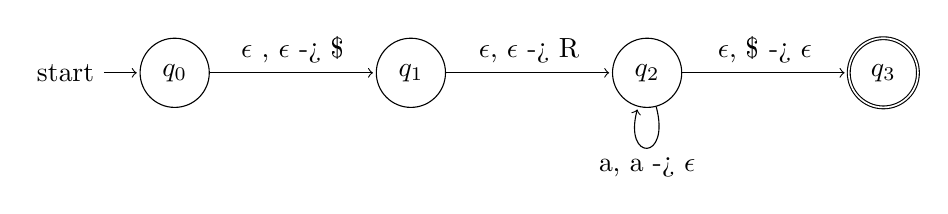
\begin{tikzpicture}[shorten >=1pt,node distance=3cm,on grid,auto] 
   \node[state,initial] (q_0)   {$q_0$}; 
   \node[state] (q_1) [right=of q_0] {$q_1$}; 
   \node[state] (q_2) [right=of q_1] {$q_2$}; 
   \node[state,accepting](q_3) [right=of q_2] {$q_3$};
    \path[->] 
    (q_0) edge  node {$\epsilon$ , $\epsilon$ -> \$} (q_1)
    (q_1) edge  node {$\epsilon$, $\epsilon$ -> R} (q_2)
    (q_2) edge  node {$\epsilon $, \$ -> $ \epsilon $} (q_3) 
          edge [loop below] node {
          a, a -> $\epsilon$} (); 
\end{tikzpicture}


\section{22 march }
\subsection{assignment 2}
We can reconnize that it is two regular languages, and that when we concatinate them we get a reglang\\
sigma star is regular, \\
we can apply theom 1.49 regular langs are closed under concat.\\
\subsection{assignemnt 3}


d)\\
	use p from pumping lemma \\
    $(xy)^{3p}(x)^p$ \\
     q

\subsection{assignemnt 5}
a)
	prove by counter exsample
    \\
    ${a^ib^ic^i | i \geq 0} \cup {a,b,c}^* $
b)
	prove by counter exsample
	${a^ib^ic^i | i \geq 0} \cup {\emptyset}$
    
    


\section{10th of April}
\begin{itemize}
\item Polynomial time reductions
\item NP-completeness
\item Examples of proofs
\begin{itemize}
\item 3-SAT
\item CLIQUE
\item Vertex cover
\item Independent set
\end{itemize}
\end{itemize}


\newpage
\section{12th of April}
\subsection{CNE-SAT is NP-Complete}
\subsubsection{Cook-lenin thm}
SAT is NP-Complete\\
 	Show that:\\
    \begin{equation}
    \forall A \in NP : A \leq_p SAT,
    \end{equation}
$ A \in NP $, Let N be a polytime NTM which accepts it in time $d_1n^k +d_2$ \\
\begin{equation}
N = (Q,\sum,R, \alpha, q_o, q_accept, q_reject).
\end{equation}
Let $W = W_1W_z*W_n$ be input to A,\\
Crate (in  polytime) a boolean formula F which is satisfiable if W is accepted by N,\\
Look at accepting breach of computation tree\\
Look at sequence of configurations.
    
\subsection{Subset-sum is NP-Complete}
   
\section{17th of April}
Hamiltonian circuit is NP-complete
\\
Conclusion on NP-complete
\\
Information on theoretic lower bound technique.

\section{1st of may}
    Approximation algorithms
    \\
    $\delta$-TSP has 2-approximation algs
    \\
    For general TSP and a fixed P, $\Delta $an alg with approx p
    \\
    Vertex cover has a 2-approx alg.
    
